\section{Navigation}
\label{sec:navigation}
I implementeringen af rutenavigation måtte forskellige kortest-vej algoritmer overvejes. En passende algoritme til formålet måtte udnytte en graf over kortdataet, som blev genereret under opstart. Derudover måtte algoritmen også kunne inddrage faktorer som længden eller hastighedsgrænsen af et vejsegment i dennes vurdering af den optimale rute. Da vi ønskede at opfylde det udvidede krav til rutenavigation, om at destinationen skulle kunne ændres kontinuerligt og flydende, var det naturligt at anvende en algoritme, som genererer et kortest-vej træ. Med et sådant træ er det nemlig muligt at udvinde den korteste vej fra træets startknude og til enhver anden knude i grafen med konstant tid.

\subsection{Dijkstra}
\label{subsec:dijkstra}
Sådanne kortest-vej træs algoritmer trumfes af E. W. Dijkstras grafsøgningsalgoritme. Dijkstras algoritme tager udgangspunkt i en startknude hvorfra det resterende træ genereres. Hver af dennes tilstødende knuder besøges. Et besøg består i at sammenholde den kendte afstand mellem startknuden og den besøgte med den nye afstand. Den nye afstand ses som den kendte afstand mellem startknuden og den besøgende knude sammenlagt med afstanden mellem den besøgende og den besøgte knude. Har en knude aldrig været besøgt, er afstanden til denne blot angivet som $+\infty$, hvorfor ethvert nyt forslag er en forbedring. Besøgsrækkefølgen varetages af en prioritetskø, som prioriterer de tilstødende knuder med lavest afstand til startknuden højest. Betragtes \ref{fig:dijkstra1} og \ref{fig:dijkstra2} ses en graf og det resulterende træ hvorfra den korteste vej mellem startknuden og enhver anden knude er tydelig.

Indledningsvist implementerede vi Dijkstras ud fra en antagelse om, at det netop ville være hurtigst at generere et kortest-vej træ, når slutknuden måtte kunne flyttes frit. Dijkstras var som forventet resursekrævende under genereringen af træet, hvilket med en graf i Open Street Maps størrelsesorden viste sig som et uacceptabelt tidsforbrug.

\begin{figure}[ht]
	\centering
  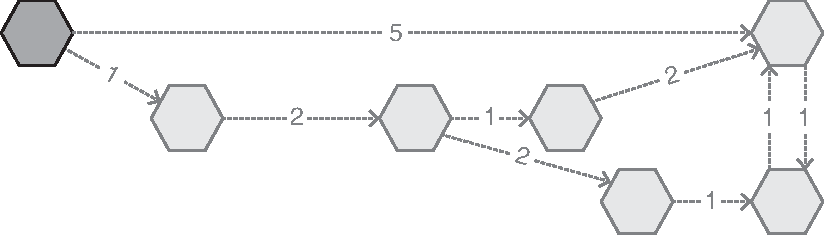
\includegraphics[width=0.7\textwidth]{dijkstra1}
  \captionsetup{width=0.8\textwidth}
  \caption{Eksempel på en vægtet orienteret graf.}
  \label{fig:dijkstra1}
\end{figure}

\begin{figure}[ht]
	\centering
  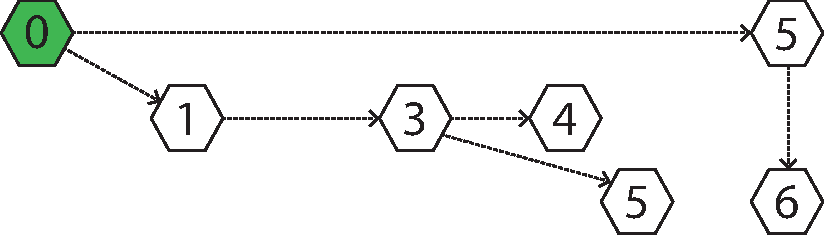
\includegraphics[width=0.7\textwidth]{dijkstra2}
  \captionsetup{width=0.8\textwidth}
  \caption{Det af Dijkstras resulterende kortest-vej træ med udgangspunkt i den grønne startknude. Distancen mellem de individuelle knuder og startknuden ses angivet.}
  \label{fig:dijkstra2}
\end{figure}

\subsection{A*}
\label{subsec:astar}
En anden algoritme, som derfor blev inddraget i overvejelserne, var A*-algoritmen. Denne generer ikke, ligesom Dijkstras, et kortest-vej træ, men finder blot den korteste vej mellem en given start- og slutknude. Da A* udvider funktionaliteten af Dijkstras algoritme, er deres adfærd meget tilsvarende. Hvor Dijkstras blot iagttager den traverserede afstand mellem den besøgte knude og startknuden, vurderer A* også en heuristik $h(x)$ for afstanden til \emph{slutknuden}. Besøgsrækkefølgen varetages stadigvæk af en prioritetskø, men nu prioriteres der efter funktionen $f(x)=g(x)+h(x)$, hvor $g(x)$ er afstanden mellem den besøgte knude og startknuden som set i Dijkstras.

I et forsøg på at forøge hastigheden af navigationsudregningen, implementerede vi således A* og sammenholdte dennes tidsforbrug med Dijkstras. A* implementeringen viste sig i praksis at være langt det hurtigste valg, selvom ændring af destinationsknuden var mere krævende.

\begin{figure}[ht]
	\centering
  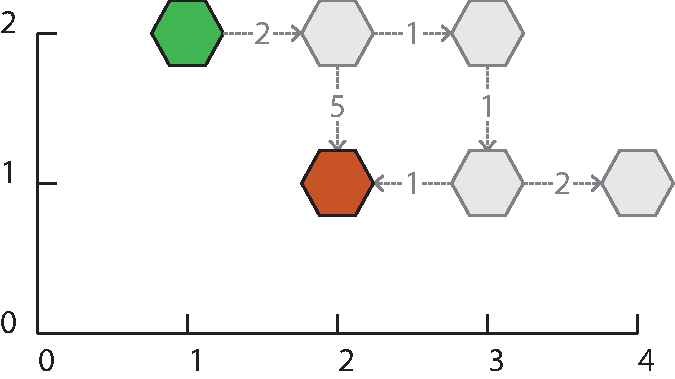
\includegraphics[width=0.6\textwidth]{astar1}
  \captionsetup{width=0.8\textwidth}
	\caption{Eksempel på en orienteret vægtet graf opstillet i et koordinatsystem som angiver distanceheuristikken. Heuristikfunktionen $h(x)$ angives som Manhattan-afstanden ved $|x_2-x_1|+|y_2-y_1|$.}
  \label{fig:astar1}
\end{figure}

\begin{figure}[ht]
	\centering
  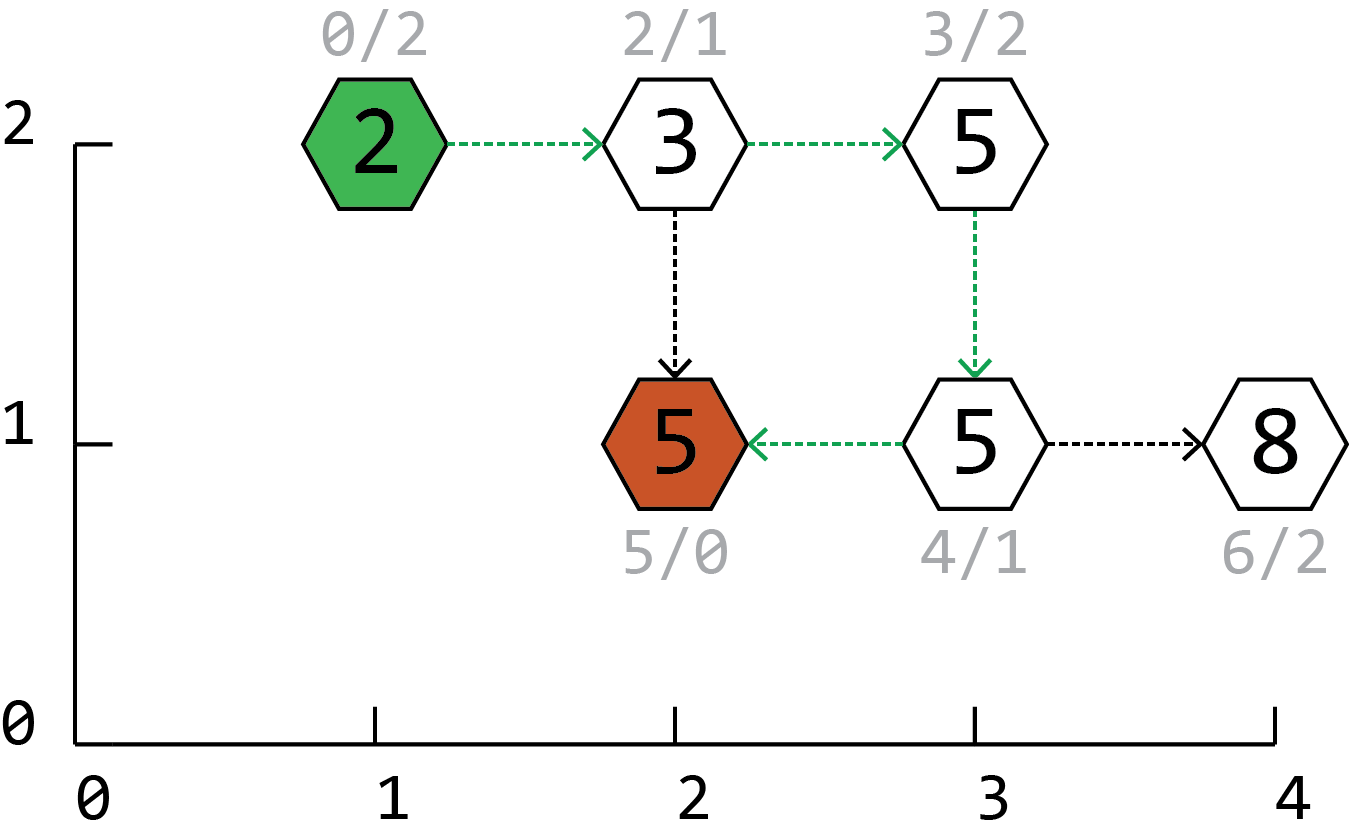
\includegraphics[width=0.5\textwidth]{astar2}
  \captionsetup{width=0.8\textwidth}
	\caption{Den af A* resulterende korteste vej mellem start- og slutknuden. Værdierne i knuderne angiver $f(x)$, mens venstre- og højresiden af skråstregen angiver henholdsvis $g(x)$ og $h(x)$. (Det er bestemt ikke en selvfølge, at samtlige knuder besøges, som er tilfældet i dette eksempel.)}
  \label{fig:astar2}
\end{figure}

\subsection{Ruteomkostninger}
\label{subsec:ruteomkostninger}
Kvaliteten af både Dijkstra og A* algoritmernes resulterende korteste vej afhænger naturligt af hvilke informationer et linjesegments længde defineres ved. Et intuitivt svar er vejens egentlige længde, hvorfor dette også blev anvendt i de indledende implementeringer. Det viste sig dog hurtigt at være en uhensigtsmæssig tilgang, da den korteste vej ikke nødvendigvis er den hurtigste. Derudover forsagede det også stor mængde kursændringer, hvilket er uønsket for både længden af rutebeskrivelsen i programmet samt for letheden af den egentlige kørsel. For at løse dette udregnedes\footnote{Kraks datasæt indeholder køretider på veje, men vi valgte at omgå disse for også at imødekomme andre datasæt. (herunder OSM).} i stedet tidsforbruget for et linjesegment.\footnote{$Tid=længde/hastighed*1.15$} Krak arbejder med en trafiktillægstid på 15\% i deres datasæt, hvilket vi har ladet vores implementering inspirere af.